\chapter{Hardware Design and System Architecture}

The OMNICAR platform is built upon a modular two-layer chassis, specifically designed to optimize the arrangement of sensors and processing units. 

Unlike traditional designs that strictly separate power and control electronics, this layout focuses on operational convenience and sensor efficiency. 

\begin{figure}[H]
    \centering
    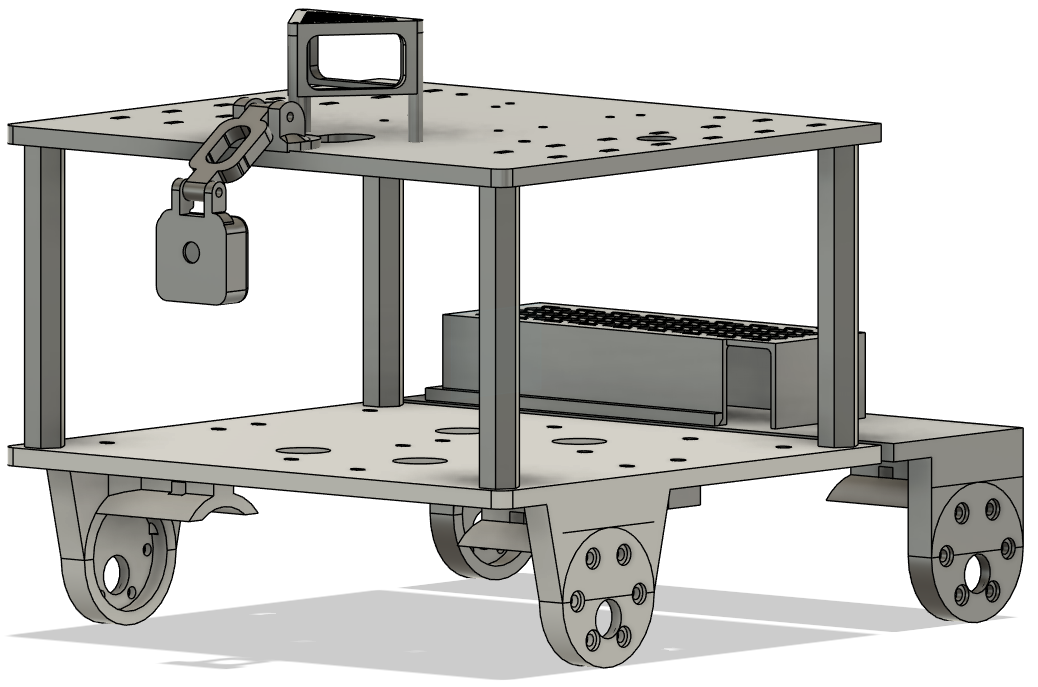
\includegraphics[width=0.8\textwidth]{IMG/Design/robot_completo.png}
    \caption{Full assembly model for 3D printing}
    \label{fig:primo_ordine}
\end{figure}

\newpage
\section{Mechanical Redesign and Optimization}
The \textbf{lower layer} houses the DC-DC converter, ESP32 microcontroller, motor drivers, and the battery, ensuring a low center of gravity for better dynamic stability. In this revision, the \textbf{motor mounts} have been significantly raised and reinforced to improve structural rigidity and better accommodate the mechanical stresses during high-torque maneuvers. Additionally, the mounts now feature dedicated slots for \textbf{nylon zip ties}, providing a secondary fastening method to ensure the motors remain perfectly aligned and secure. 

Furthermore, a custom \textbf{battery Case} has been designed and implemented. It utilizes a \textbf{sliding rail mechanism} that allows the Case to snap into place securely without the need for screws. This design choice significantly improves the robot's usability, allowing for rapid battery replacement during testing phases.

The \textbf{lower layer} houses the ESP32 microcontroller, motor drivers, and battery, keeping the center of mass low and reducing the wiring distance to the motors. 
% components of lower layer 
\begin{figure}[H]
    \centering
    \begin{minipage}[b]{0.4\textwidth}
        \centering
        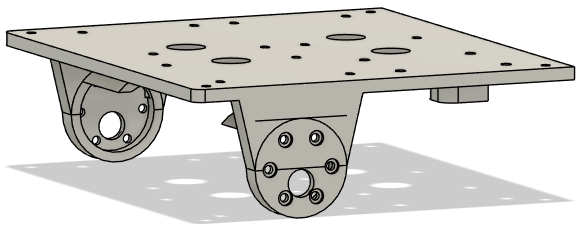
\includegraphics[width=\textwidth]{IMG/Design/ly1_front.png}
        \caption*{Front lower layer}
    \end{minipage}
    \hfill
    \begin{minipage}[b]{0.4\textwidth}
        \centering
        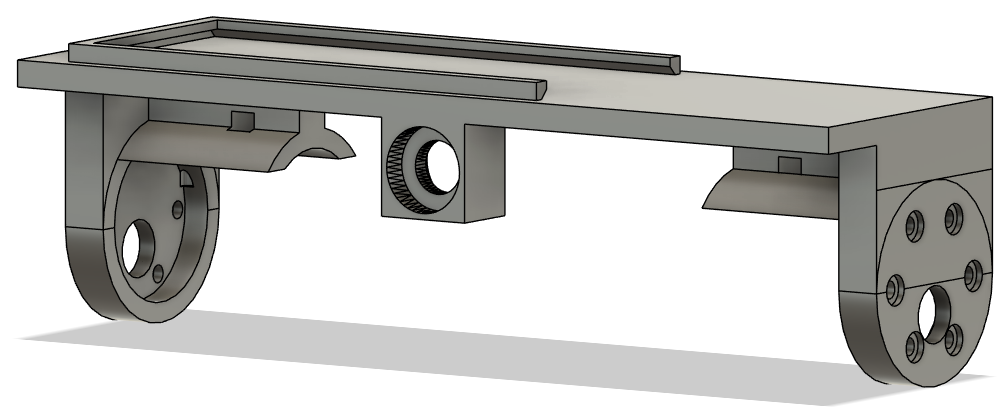
\includegraphics[width=\textwidth]{IMG/Design/ly1_back.png}
        \caption*{Back lower layer}
    \end{minipage}
    \hfill
    \begin{minipage}[b]{0.4\textwidth}
        \centering
        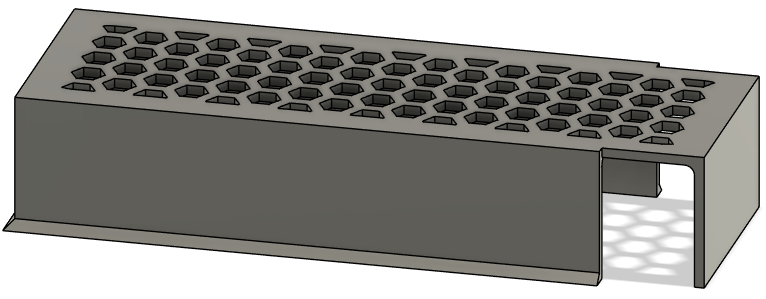
\includegraphics[width=\textwidth]{IMG/Design/cover_batteria.png}
        \caption*{Battery Case}
    \end{minipage}
    \caption{Lower layer components}
    \label{fig:Lower layer components}
\end{figure}

\begin{figure}[H]
    \centering
    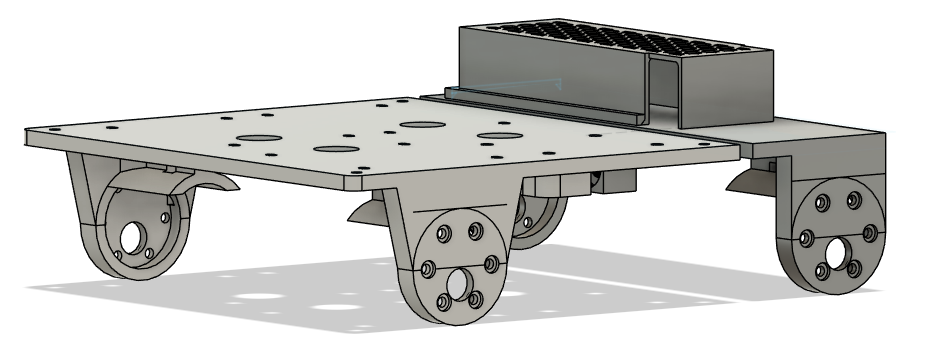
\includegraphics[width=0.7\textwidth]{IMG/Design/ly1_completo.png}
    \caption{Lower layer assembled}
    \label{fig:Lower layer assembled}
\end{figure}

\newpage
The \textbf{upper layer} is dedicated to the high-level navigation suite. It provides an elevated platform for the LIDAR and the Pi Camera, ensuring a clear line of sight for environment mapping and obstacle detection. Additionally, this placement allows the Raspberry Pi 5 to be located directly adjacent to the LIDAR, simplifying the USB/Serial connection and reducing electromagnetic interference in high-speed data transmission.

\begin{figure}[H]
    \centering
    \begin{minipage}[b]{0.60\textwidth}
        \centering
        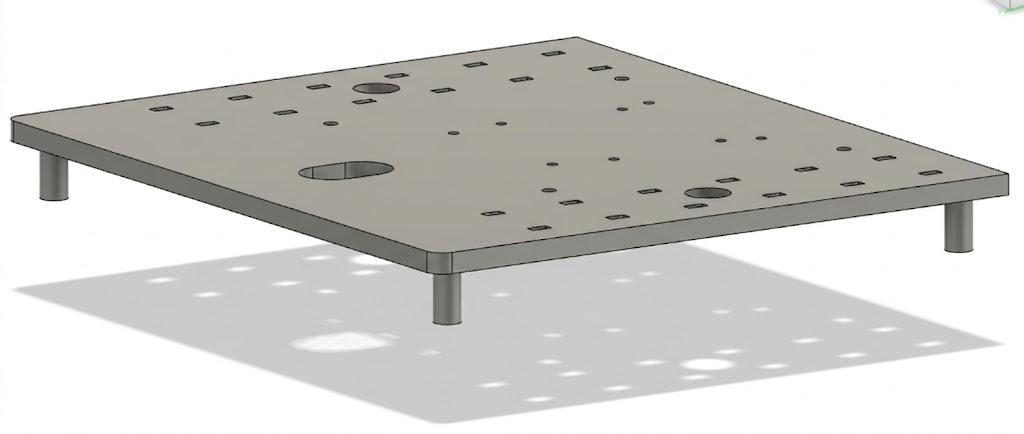
\includegraphics[width=\textwidth]{IMG/Design/ly2_piastra.jpg}
        \caption*{Upper layer}
    \end{minipage}
    \hfill
    \begin{minipage}[b]{0.28\textwidth}
        \centering
        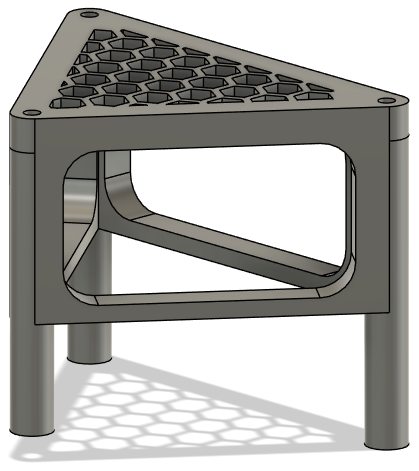
\includegraphics[width=\textwidth]{IMG/Design/lidar_support.png}
        \caption*{Lidar support}
    \end{minipage}
    \hfill
    \begin{minipage}[b]{0.28\textwidth}
        \centering
        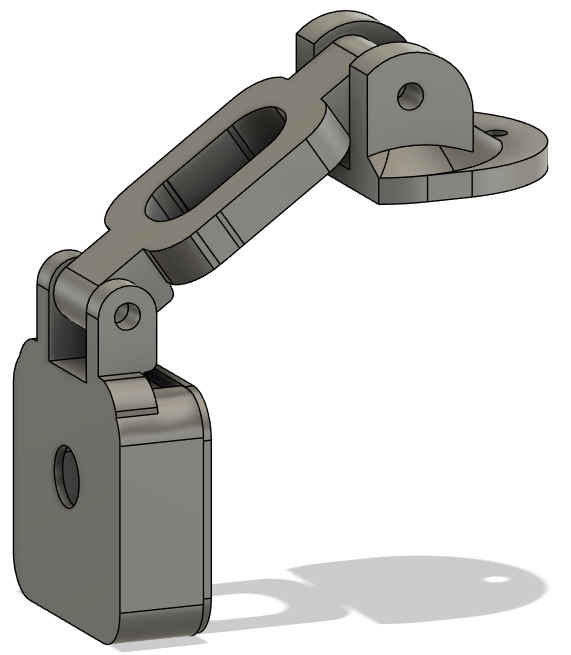
\includegraphics[width=\textwidth]{IMG/Design/stand_pi_camera.png}
        \caption*{Stand pi camera}
    \end{minipage}
    \caption{Upper layer components}
    \label{fig:Upper layer components}
\end{figure}


\begin{figure}[H]
    \centering
    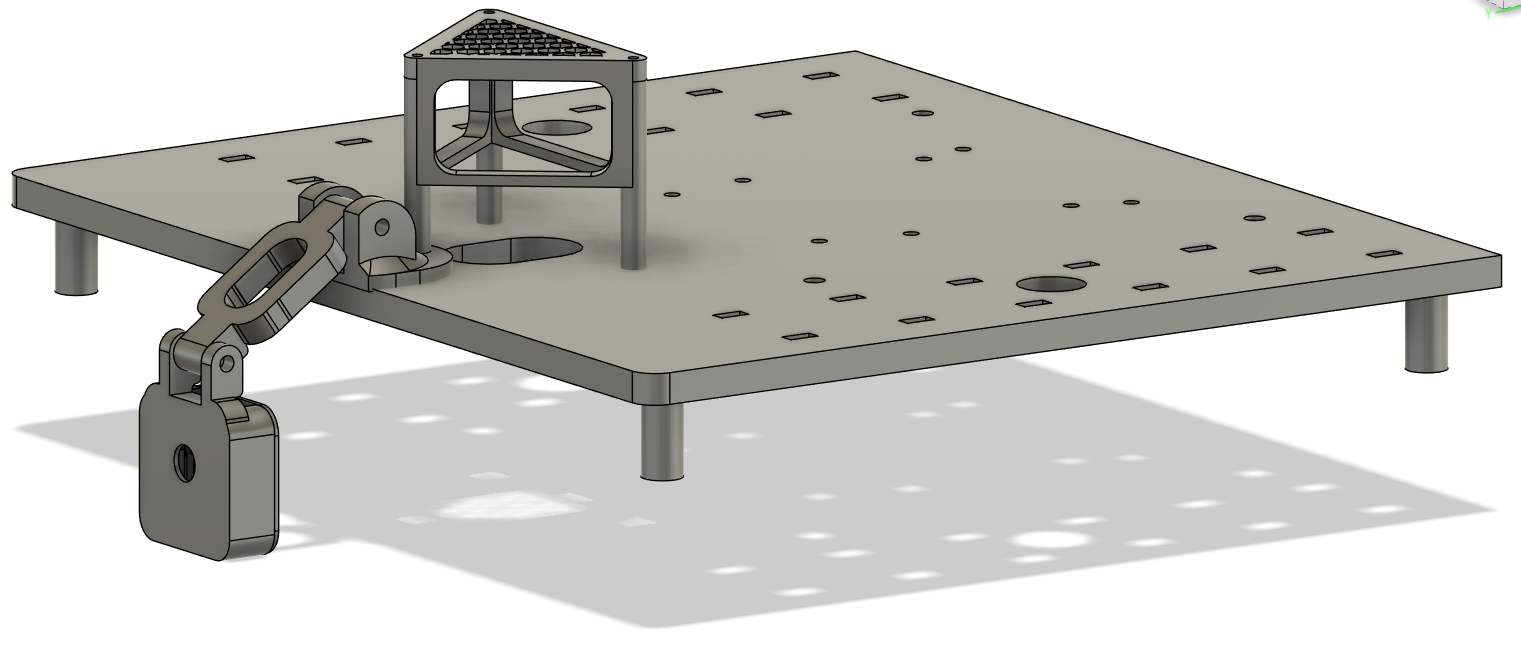
\includegraphics[width=0.7\textwidth]{IMG/Design/ly2_completo.png}
    \caption{Bottom layer assembled}
    \label{fig:Lower layer assembled}
\end{figure}

To facilitate the development and validation of the control algorithms, a custom-designed support stand was developed for the OMNICAR platform. This component proved to be \textbf{essential during the debugging and initial testing phases}, particularly for verifying the response of the four independent motors.

By elevating the chassis, the stand allowed the wheels to rotate freely in a "no-load" condition. 
This setup was extremely useful for:
\begin{itemize}
    \item Calibrating the high-resolution encoders without the interference of ground friction.
    \item Validating the mapping of PWM signals to the MDD10A motor drivers.
    \item Identifying potential hardware asymmetries or wiring issues before conducting field tests.
\end{itemize}

The mechanical design follows an \textbf{ergonomic and minimalist approach}. A key feature of the structure is the integration of a hollow central grip. This design choice was not only functional, providing an easy point of handle for moving the robot and stand together, but also strategically \textbf{economical}. By incorporating this empty space, the total volume of 3D-printing filament was significantly reduced, leading to faster production times and lower material costs without compromising the structural integrity required to support the robot's weight.

\begin{figure}[H]
    \centering
    \begin{minipage}[b]{0.48\textwidth}
        \centering
        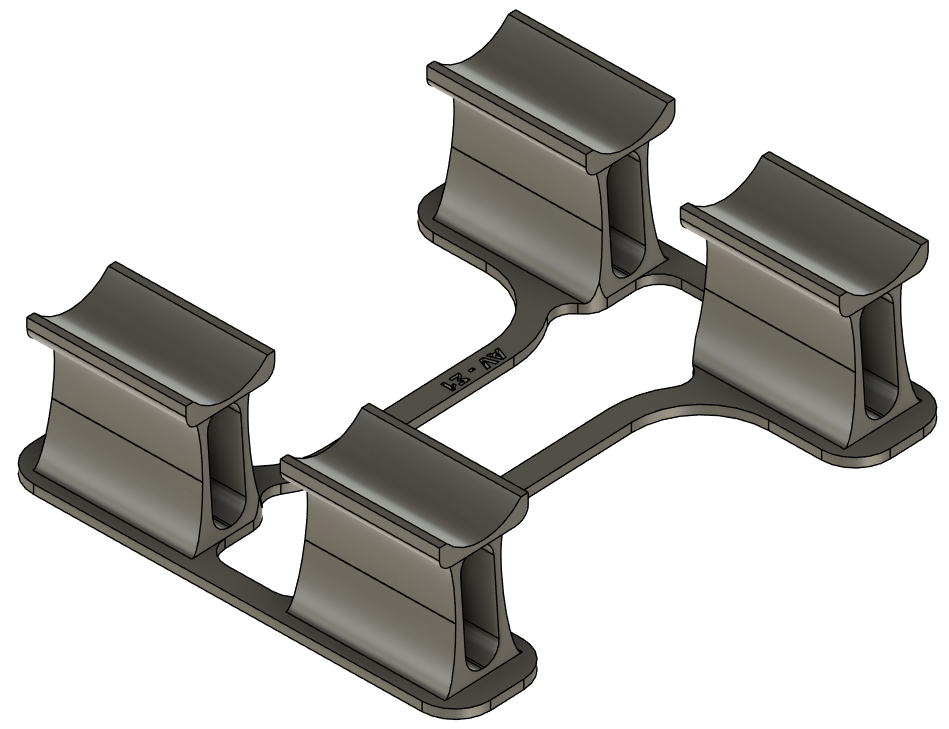
\includegraphics[width=\textwidth]{IMG/Design/Stand.png}
        \caption*{Stand}
    \end{minipage}
    \hfill
    \begin{minipage}[b]{0.48\textwidth}
        \centering
        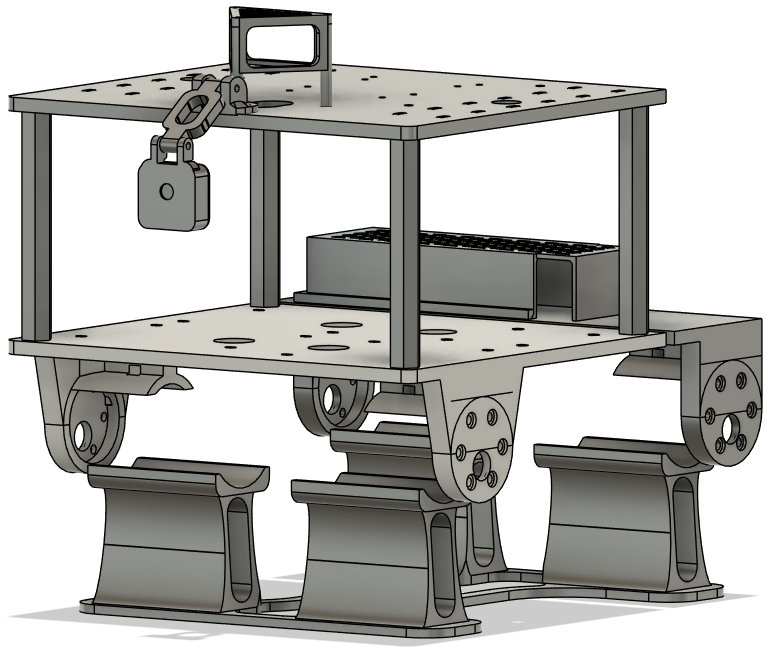
\includegraphics[width=\textwidth]{IMG/Design/Omnicar_with_Stand.png}
        \caption*{Omnicar and Stand assembled}
    \end{minipage}
    \label{fig:Omnicar and Stand assembled}
    \label{fig:Custom-designed test stand for the OMNICAR platform}
\end{figure}

\section{Actuators, Sensors and Electronic System}
The motion system is powered by four \textbf{Pololu 37Dx73L mm} metal gearmotors. These actuators are equipped with integrated 64 CPR quadrature encoders which, through the gear ratio, provide a high-resolution feedback of approximately \textbf{1200 counts per revolution}. This level of precision is fundamental for maintaining accurate odometry and ensuring stable trajectory tracking.

To manage the complex power requirements of both high-level processing and low-level actuation, the robot integrates a robust power distribution stage. A high-capacity \textbf{300W 20A DC-DC buck converter} is utilized to step down the battery voltage, providing a stabilized power rail for the most demanding components like encoders, \textbf{Raspberry Pi 5} and the \textbf{LIDAR} sensor.

To manage the complex power requirements of both high-level processing and low-level actuation, the robot's electrical architecture integrates a robust power distribution stage. The system is primary energized by a \textbf{Combo Battery 5000mAh 11.1V 3S1P} LiPo battery, chosen for its high energy density and discharge rate capabilities. To interface this source with the onboard electronics, a high-capacity \textbf{300W 20A DC-DC buck converter} is utilized to step down the battery voltage. This regulation provides a stabilized power rail for the most demanding components, including the high-resolution encoders, the \textbf{Raspberry Pi 5} central processing unit, and the \textbf{LIDAR} sensor, ensuring operational stability even during high-torque motor maneuvers.

\begin{figure}[H]
        \centering
        \begin{minipage}[b]{0.30\textwidth}
            \centering
            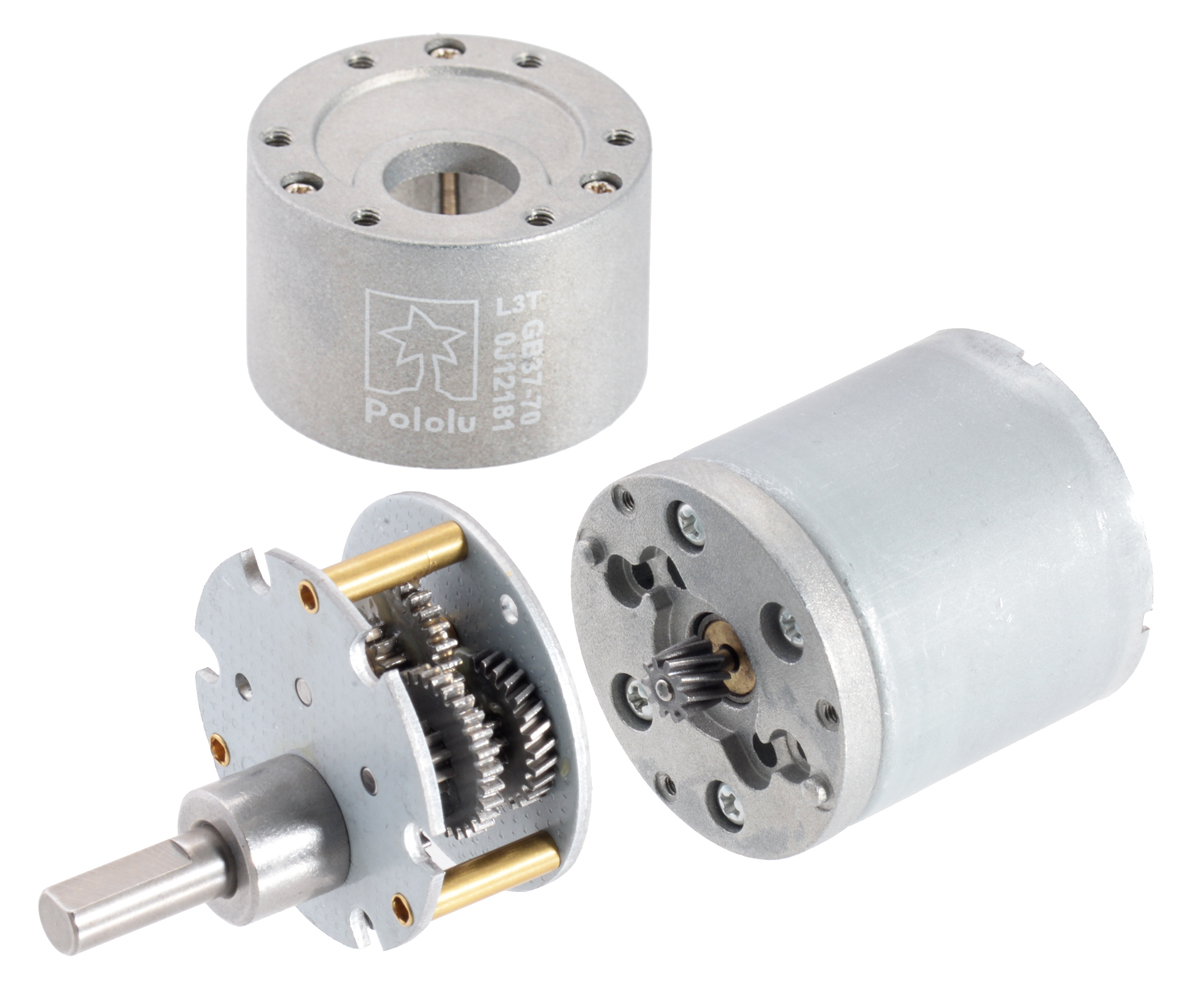
\includegraphics[width=\textwidth]{IMG/Componenti_Ele/pololu_motor.jpeg}
            \caption*{Pololu Metal DC Gearmotors}
        \end{minipage}
        \hfill
        \begin{minipage}[b]{0.30\textwidth}
            \centering
            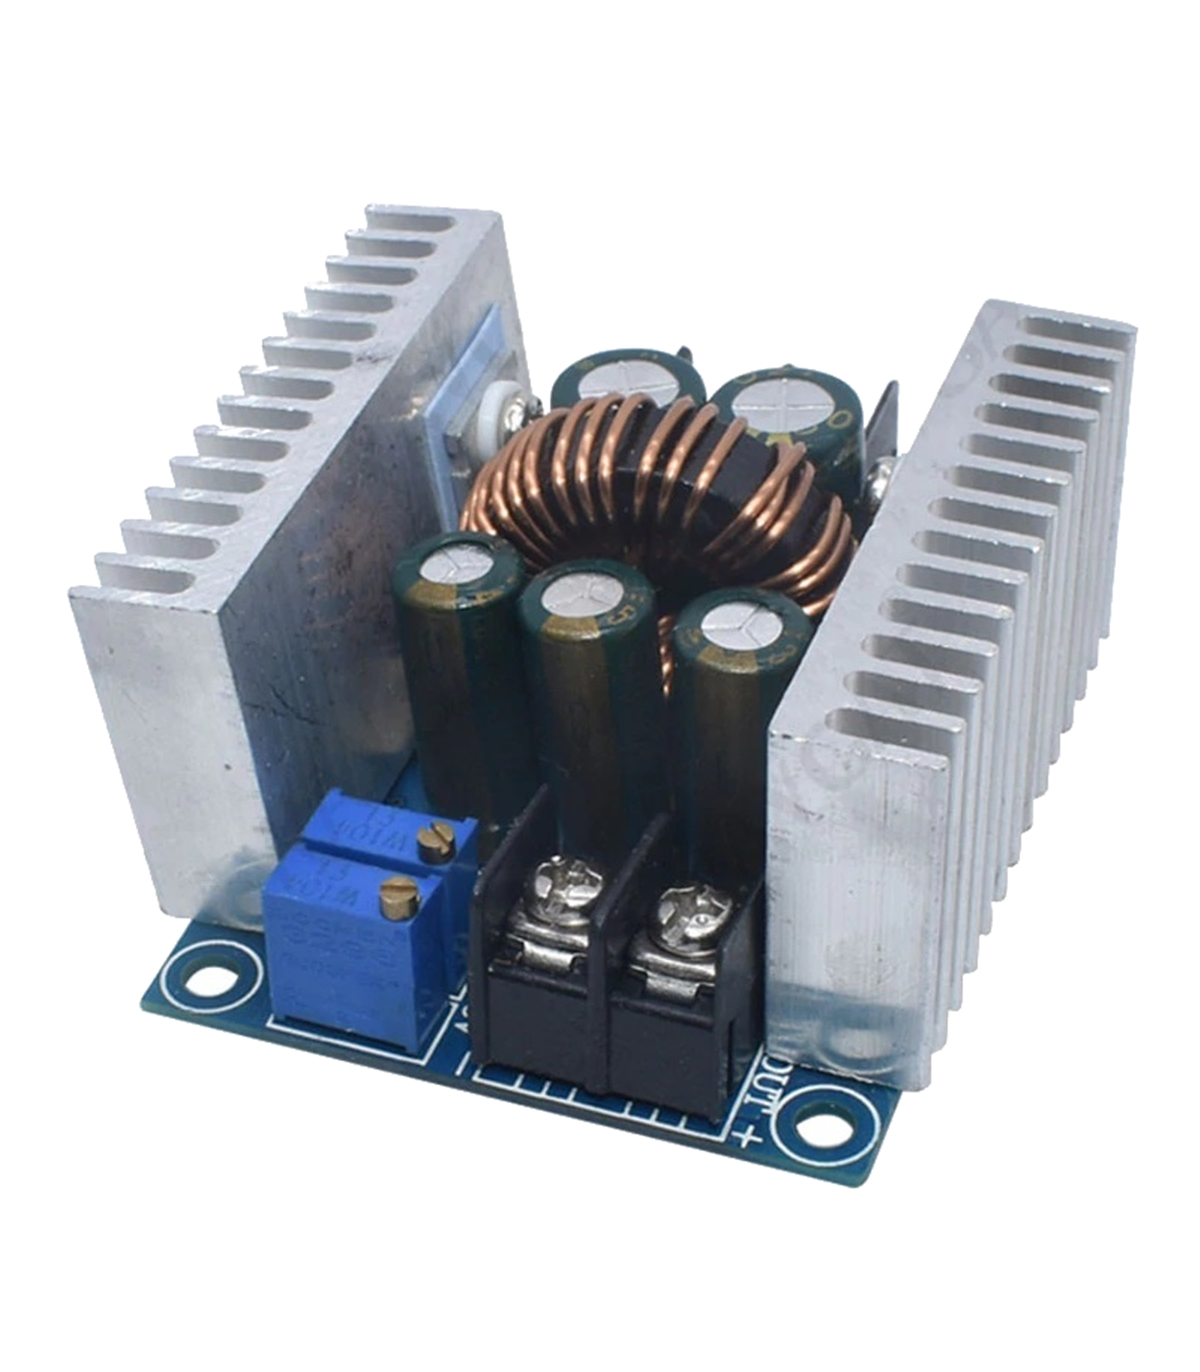
\includegraphics[width=\textwidth]{IMG/Componenti_Ele/DC_DC_Conv.jpg}
            \caption*{DC-DC Buck Converter }
        \end{minipage}
        \hfill
        \begin{minipage}[b]{0.50\textwidth}
            \centering
            
\includegraphics[width=\textwidth]{IMG/Componenti_Ele/battery_11_1.jpg}
    \caption{Battery 5000mAh 11.1V 3S1P}
        \end{minipage}
        \label{fig:12 Volt Components}
\end{figure}

\begin{comment}
\begin{figure}[H]
    \centering
    
\includegraphics[width=0.40\textwidth]{IMG/Componenti_Ele/battery_11_1.jpg}
    \caption{Battery 5000mAh 11.1V 3S1P}
    \label{fig:Battery 5000mAh 11.1V 3S1P}
\end{figure}
\end{comment}

The control architecture is divided into two main functional blocks:

\begin{itemize}
    \item \textbf{Low-Level Control:} The core of this subsystem is an \textbf{ESP32-WROOM} microcontroller, chosen for its dual-core architecture and dedicated hardware peripherals. The ESP32 handles the real-time execution of the control loop, utilizing its hardware timers for precise \textbf{PWM generation} and its \textbf{Pulse Counter (PCNT)} modules for efficient, high-frequency encoder reading.
    
    \begin{figure}[H]
    \centering
    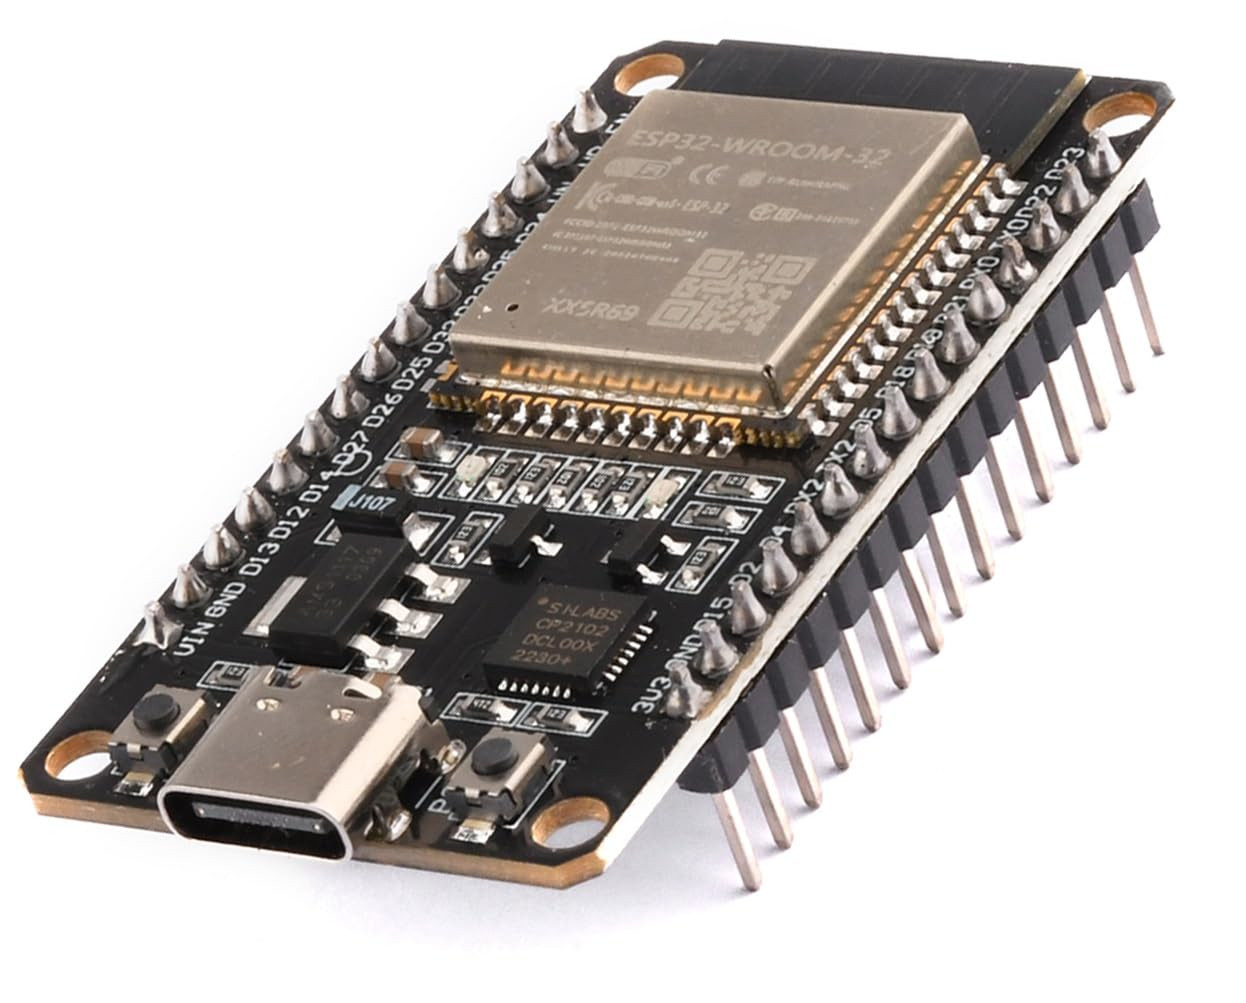
\includegraphics[width=0.45\textwidth]{IMG/Componenti_Ele/esp32.jpg}
    \caption{ESP32}
    \label{fig:ESP32}
    \end{figure}

    \item \textbf{Motor Actuation:} The microcontroller interfaces with two \textbf{MDD10A} dual-channel motor drivers. This setup allows for independent control of each wheel's speed and direction through a PWM/DIR interface, creating a closed-loop system where the ESP32 simultaneously commands the motors and monitors wheel position.
    
    \begin{figure}[H]
    \centering
    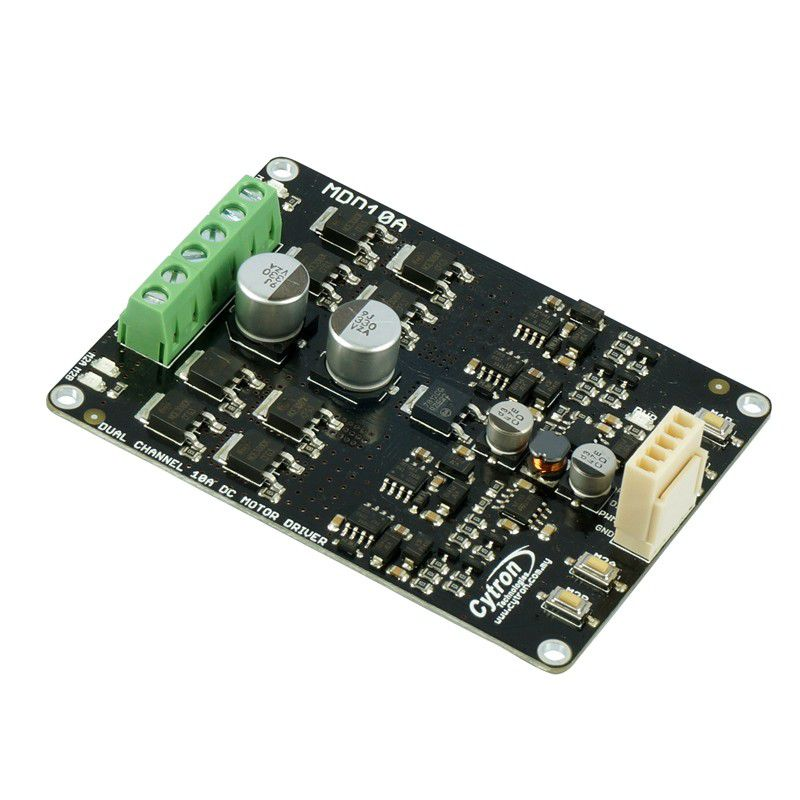
\includegraphics[width=0.45\textwidth]{IMG/Componenti_Ele/driver_MD10A.jpeg}
    \caption{Driver MDD10A}
    \label{fig:Driver MDD10A}
    \end{figure}
    
    \item \textbf{High-Level Navigation:} A \textbf{Raspberry Pi 5} serves as the primary computational unit, processing data from the \textbf{LIDAR} and \textbf{Pi Camera} to perform environment mapping and path planning, subsequently communicating target velocities to the ESP32.
    \begin{figure}[H]
        \centering
        \begin{minipage}[b]{0.43\textwidth}
            \centering
            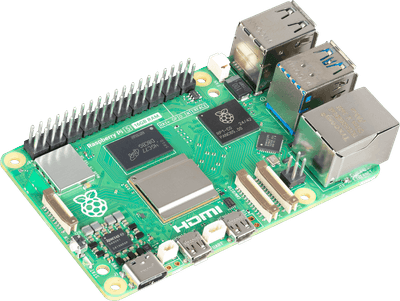
\includegraphics[width=\textwidth]{IMG/Componenti_Ele/raspberry_pi5.png}
            \caption*{Upper layer}
        \end{minipage}
        \hfill
        \begin{minipage}[b]{0.43\textwidth}
            \centering
            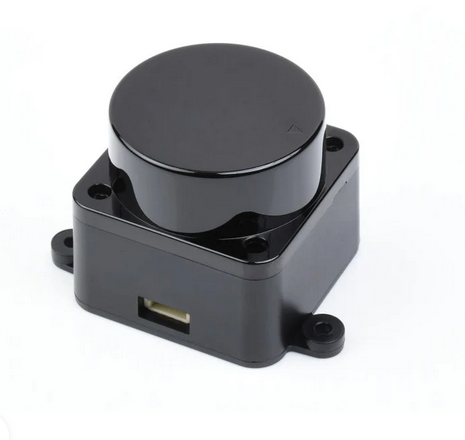
\includegraphics[width=\textwidth]{IMG/Componenti_Ele/Lidar.png}
            \caption*{Lidar}
        \end{minipage}
    \end{figure}
    
\end{itemize}

\section{Electrical Design and Connection Architecture}

The design of the entire electrical system for the OMNICAR platform was developed using the \textbf{EasyEDA online editor}. Thanks to the integrated component libraries, it was possible to model the power interfaces of the motor drivers and the logical connections of the microcontroller, ensuring a high degree of fidelity between the theoretical design and the final hardware.

The result of this phase is the \textbf{general electrical schematic} of the platform, illustrated in Figure \ref{fig:connection_architecture_easyeda}, which serves as the blueprint for the entire control and power distribution system. The schematic is structured to isolate the high-current power lines intended for the motors from the 3.3V and 5V logic signals required for the control logic and sensors. This separation is crucial to prevent cross-talk and ensure the stability of the feedback signals from the encoders during the robot's maximum acceleration phases.

\subsection{Physical Layout and Layer Organization}

The physical organization of the hardware follows a layered logic to optimize space and weight distribution:

\begin{itemize}
    \item \textbf{Lower Layer (Base):} This level constitutes the electromechanical heart of the robot. It houses the \textbf{ESP32 DevKit}, the four \textbf{MDD10A} drivers, and the power distribution system. Placing these at the base allows for a lower center of gravity and reduces the length of the wiring to the motors, minimizing electromagnetic interference (EMI).
    \item \textbf{Upper Layer (Sensor Deck):} To ensure a field of view free from obstacles, the \textbf{Raspberry Pi 5}, the \textbf{LIDAR} sensor, and the \textbf{Pi Camera} are installed on the upper structure. This configuration protects the processing units from the heat generated by the drivers and provides an optimal perspective for navigation and vision algorithms.
\end{itemize}

\subsection{ESP32 Pinout and Wiring Specification}

The \textbf{ESP32-WROOM} microcontroller was selected for its high-performance architecture, capable of simultaneously managing non-linear control loops and high-frequency encoder readings. The connection configuration was designed to maximize the use of dedicated hardware peripherals, such as PWM (LEDC) and Pulse Counters (PCNT). The detailed mapping of these connections is provided in Table \ref{tab:esp32_pinout}.

\subsection{Pin Selection Justification}

The pin assignment was guided by specific technical constraints to ensure system reliability:

\begin{enumerate}
    \item \textbf{High-Resolution Feedback:} With encoders providing 1200 pulses per revolution, it was necessary to use pins compatible with the \textbf{PCNT} hardware peripheral. Pins 34-39 were specifically chosen for the rear encoders because, as "Input-Only" pins, they lack internal pull-up/pull-down circuitry that could interfere with the signal, thus guaranteeing digital integrity without the risk of output conflicts.
    \item \textbf{PWM Generation:} The \textbf{LEDC} peripheral was utilized to control the MDD10A drivers. The assigned pins allow for independent, hardware-timed PWM signals, which are essential for maintaining a deterministic response in holonomic kinematics.
    \item \textbf{Communication Integrity:} Predefined hardware \textbf{UART} pins were reserved for data exchange with the Raspberry Pi 5, supporting baud rates up to 115200 bps for real-time transmission of velocities and poses.
\end{enumerate}

\begin{comment}
    \item \textbf{Boot Stability:} So-called "strapping pins" (such as GPIO 0, 2, 5, 12, and 15) and pins linked to the internal SPI flash were avoided where possible to prevent firmware boot errors or unexpected behavior during power-up under full-load conditions.
\end{comment}

% --- Final Figures and Tables ---
\begin{table}[H]
\centering
\caption{ESP32 Complete Pinout for OMNICAR Motion Control}
\label{tab:esp32_pinout}
% Definiamo un colore leggero per le righe alternate (grigio al 90% di bianco)
\rowcolors{2}{gray!10}{white} 
\begin{tabularx}{\textwidth}{l c c X} % X è una colonna che si espande automaticamente
\toprule
\textbf{Function} & \textbf{GPIO} & \textbf{Signal Type} & \textbf{Project Description} \\ 
\midrule
Main Power Supply & VIN & Power (+5V) & Main DC input \\
Common Ground     & GND & GND          & Common return \\
\addlinespace % Piccolo spazio extra per separare i gruppi
Motor FL PWM      & 13  & Output (LEDC) & Front-Left speed control \\
Motor FL DIR      & 12  & Output        & Front-Left direction \\
Motor FR PWM      & 14  & Output (LEDC) & Front-Right speed control \\
Motor FR DIR      & 27  & Output        & Front-Right direction \\
Motor RL PWM      & 26  & Output (LEDC) & Rear-Left speed control \\
Motor RL DIR      & 25  & Output        & Rear-Left direction \\
Motor RR PWM      & 33  & Output (LEDC) & Rear-Right speed control \\
Motor RR DIR      & 32  & Output        & Rear-Right direction \\
\addlinespace
Encoder FL (A/B)  & 16 / 17 & Input (PCNT) & Front-Left feedback \\
Encoder FR (A/B)  & 5 / 18 & Input (PCNT) & Front-Right feedback \\
Encoder RL (A/B)  & 19 / 21 & Input (Only) & Rear-Left feedback \\
Encoder RR (A/B)  & 22 / 23 & Input (Only) & Rear-Right feedback \\
\bottomrule
\end{tabularx}
\end{table}

\newgeometry{margin=3cm} % Stringe i margini solo per questa pagina
\begin{figure}[p]
    \centering
    \vspace*{\fill}
    \makebox[\textwidth][c]{%
        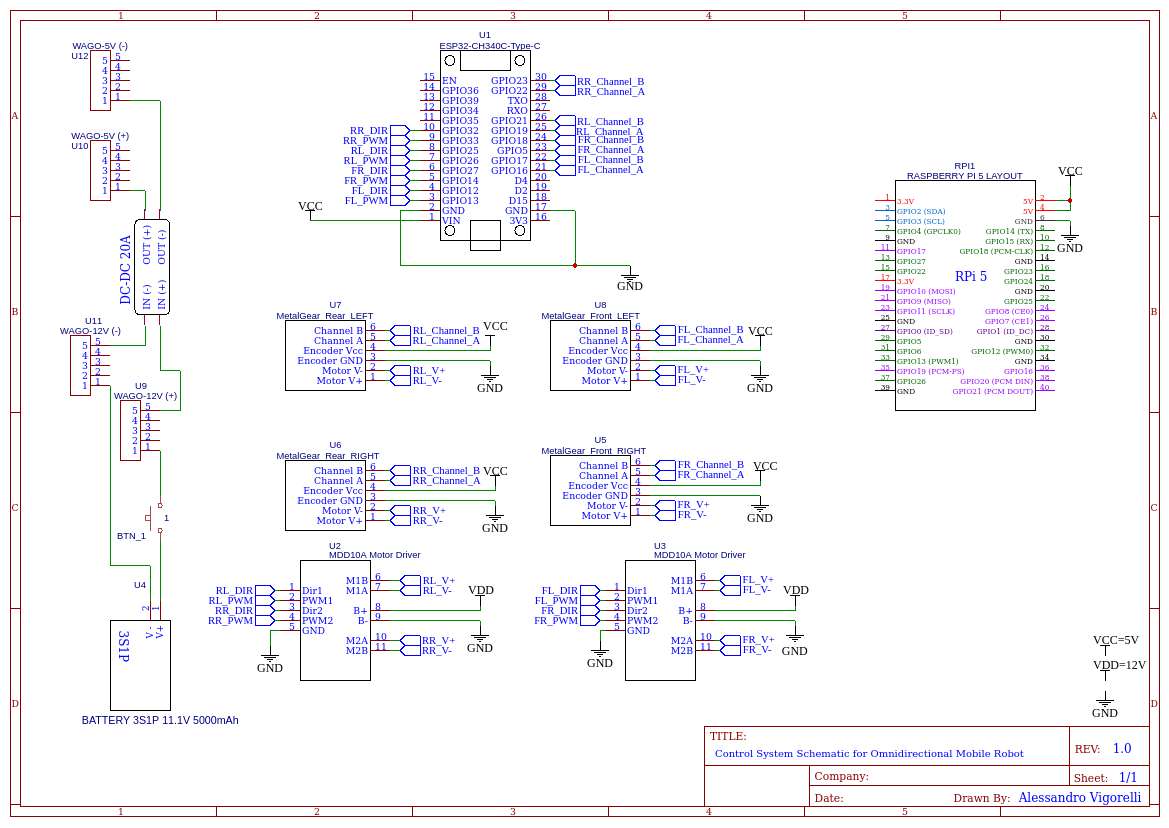
\includegraphics[height=1.1\textwidth, angle=90, origin=c]{IMG/Design/Schematic_OMNICAR.png}
    }
    \vspace*{\fill}
    \caption{Detailed Connection Architecture designed in EasyEDA}
    \label{fig:connection_architecture_easyeda}
\end{figure}
\restoregeometry % Torna ai margini normali nella pagina successiva